%%%%%%%%%%%%%%%%%%%%%%%%%%%%%%%%%%%%%%%%%%%%%%%%%%%%%%%%%%%%%%%%%%%%%%%%%%%%%%%%
%2345678901234567890123456789012345678901234567890123456789012345678901234567890
%        1         2         3         4         5         6         7         8

\documentclass[letterpaper, 10 pt, conference]{IEEEconf}  % Comment this line out
                                                          % if you need a4paper
%\documentclass[a4paper, 10pt, conference]{ieeeconf}      % Use this line for a4
                                                          % paper

% See the \addtolength command later in the file to balance the column lengths
% on the last page of the document
\usepackage[table,xcdraw]{xcolor}
\usepackage{amsmath,amsthm,amssymb}
\usepackage{float}
\usepackage[pdftex]{graphicx}
\usepackage{color}
\usepackage{mathtools}          %loads amsmath as well
\usepackage{titlesec}

\titlespacing\section{0pt}{12pt plus 4pt minus 2pt}{0pt plus 2pt minus 2pt}
\titlespacing\subsection{0pt}{12pt plus 4pt minus 2pt}{0pt plus 2pt minus 2pt}
\titlespacing\subsubsection{0pt}{12pt plus 4pt minus 2pt}{0pt plus 2pt minus 2pt}

% The following packages can be found on http:\\www.ctan.org
%\usepackage{graphics} % for pdf, bitmapped graphics files
%\usepackage{epsfig} % for postscript graphics files
%\usepackage{mathptmx} % assumes new font selection scheme installed
%\usepackage{times} % assumes new font selection scheme installed
%\usepackage{amsmath} % assumes amsmath package installed
%\usepackage{amssymb}  % assumes amsmath package installed

\title{\LARGE \bf ECE 527 SoC Design Machine Problem 1}

%\author{ \parbox{3 in}{\centering Huibert Kwakernaak*
%         \thanks{*Use the $\backslash$thanks command to put information here}\\
%         Faculty of Electrical Engineering, Mathematics and Computer Science\\
%         University of Twente\\
%         7500 AE Enschede, The Netherlands\\
%         {\tt\small h.kwakernaak@autsubmit.com}}
%         \hspace*{ 0.5 in}
%         \parbox{3 in}{ \centering Pradeep Misra**
%         \thanks{**The footnote marks may be inserted manually}\\
%        Department of Electrical Engineering \\
%         Wright State University\\
%         Dayton, OH 45435, USA\\
%         {\tt\small pmisra@cs.wright.edu}}
%}

\author{Andrew Smith(atsmith3) and Thomas Furlong(tfurlon2)}% <-this % stops a space
\begin{document}



\maketitle
\thispagestyle{empty}
\pagestyle{empty}


%%%%%%%%%%%%%%%%%%%%%%%%%%%%%%%%%%%%%%%%%%%%%%%%%%%%%%%%%%%%%%%%%%%%%%%%%%%%%%%%
\section{INTRODUCTION}

This MP was designed to become familiar with the Xilinx tools. We set up the development environment on a lightweight ubuntu distribution and interfaced with the ZedBoard. We walked through the compilation process as well as practiced incorporating the Zynq hard IP core into the design by generating a Board Support Package and writing software in the Xilinx SDK.

\section{Part A}
\subsection{Description}
For the first part of the MP we had to write a small verilog module for the programmable logic fabric portion of the Xilinx Zinq 7000 chip. This module needs to read the positions of the 8 on board switches and display the switch position on the 8 user LEDs. The switch status was displayed on the LEDs after 3 clock cycles and the center button was used as a reset.

\subsection{Assumptions}
We did not have to make any assumptions for this part of the MP as the directions were very straight forward.

\subsection{System Configuration}
The part A of the machine problem was very simple so we only needed one module in the programmable logic fabric. This module took in inputs from the switches, a single input from the reset button, and a clock. The module output a vector to the LEDs containing information on the switch state. The module contained three buffering registers to ensure that the switch state appeared on the LEDs after exactly 3 clock cycles. The module is shown in figure 1.

\begin{figure}[thpb]
   \centering
   \parbox{3in}{\centering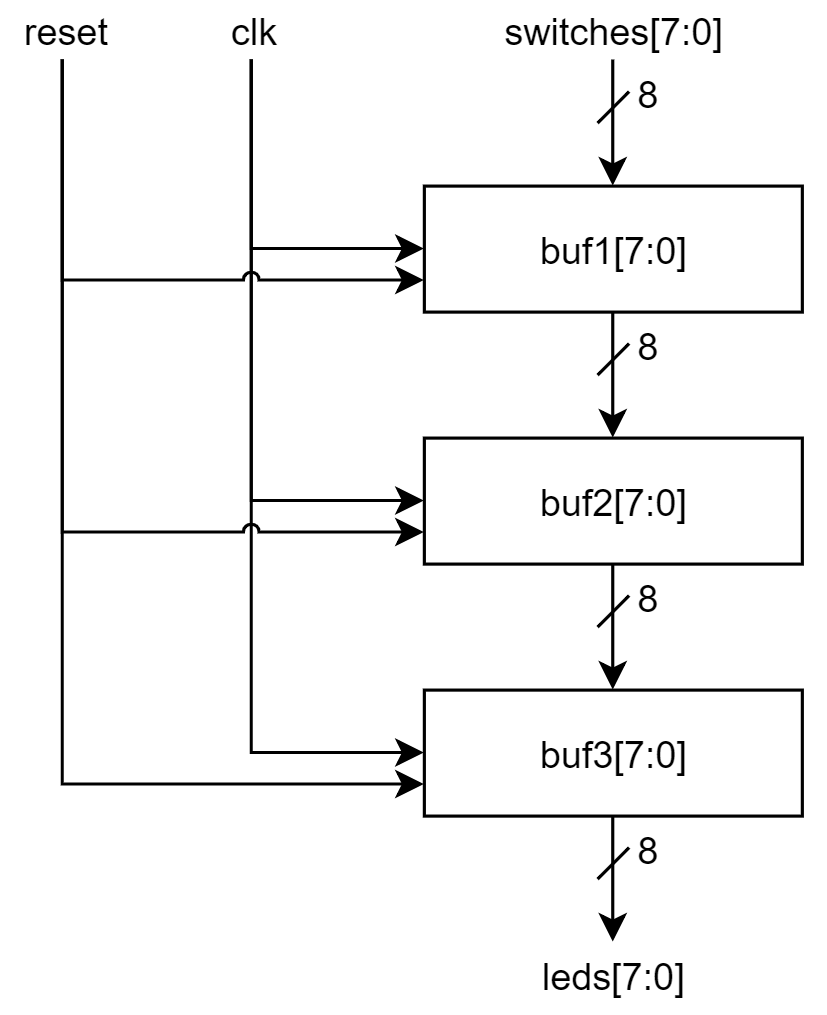
\includegraphics[scale=0.25]{img/mp1a_diagram.PNG}}
   \caption{Block Diagram for Part A}
   \label{figurelabel}
\end{figure}

\subsection{Entities}
\begin{table}[H]
\begin{tabular}{|l|l|}
\hline
\rowcolor[HTML]{EFEFEF} 
Entity      & Description                           \\ \hline
basic\_i\_o & Hardware top level, contains pipeline \\ \hline
\end{tabular}
\end{table}

\subsection{Design}
When designing we only considered one solution. Using a pipeline to transfer switch state information to the LEDs. This would ensure that the LEDs were updated with switch information after exactly 3 cycles for every change in the switches. Had we used a counter or other option it would have more complex logic and been harder to guarantee the LEDs were updated after 3 cycles.

\subsection{Performance}
This was a very small design and it took up very little resources on the Zinq 7000. The usage is shown in the table below. Figure 2 shows how the design was implemented on the device.
\begin{table}[H]
\centering
\caption{Resource Usage Part A}
\label{table_example}
\begin{tabular}{|l|r|r|r|}
\hline
\rowcolor[HTML]{EFEFEF} 
Resource & \multicolumn{1}{l|}{\cellcolor[HTML]{EFEFEF}Utilization} & \multicolumn{1}{l|}{\cellcolor[HTML]{EFEFEF}Available} & \multicolumn{1}{l|}{\cellcolor[HTML]{EFEFEF}Utilization \%} \\ \hline
LUT      & 1                                                        & 53200                                                  & 0.01                                                        \\ \hline
FF       & 24                                                       & 106400                                                 & 0.02                                                        \\ \hline
IO       & 18                                                       & 200                                                    & 9.00                                                        \\ \hline
BUFG     & 1                                                        & 32                                                     & 3.13                                                        \\ \hline
\end{tabular}
\end{table}

\begin{figure}[thpb]
   \centering
   \parbox{3in}{\centering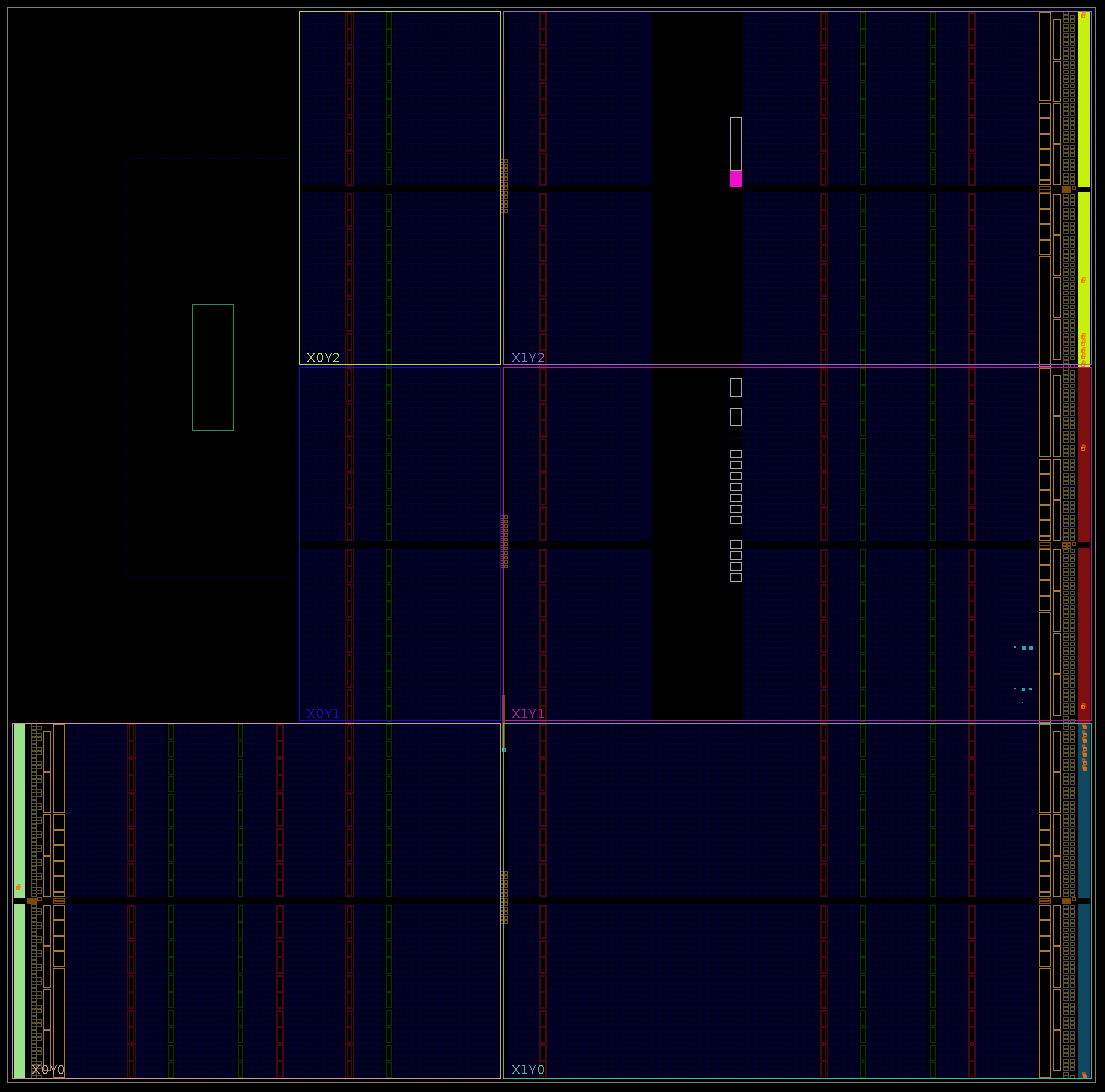
\includegraphics[scale=0.35]{img/mp1a_device.PNG}}
   \caption{Device Mapping for Part A}
   \label{figurelabel}
\end{figure}

Because this design used minimal logic most of the power consumed by the device was static power. As the transistors were mostly siting idle across the programmable logic fabric.

\begin{table}[H]
\centering
\caption{Resource Usage Part A}
\label{table_example}
\begin{tabular}{|l|r|}
\hline
\rowcolor[HTML]{EFEFEF} 
Type    & \multicolumn{1}{l|}{\cellcolor[HTML]{EFEFEF}Power} \\ \hline
Static  & 0.122 W                                            \\ \hline
Dynamic & 0.007 W                                            \\ \hline
\textbf{Total} & \textbf{0.129 W}                            \\ \hline
\end{tabular}
\end{table}

Due to the design small size the router did not have a problem satisfying the timing constraints of the clock. Shown below is some of the timing information from the timing report.

\begin{table}[H]
\centering
\caption{Timing Report Part A}
\label{table_example}
\begin{tabular}{|l|l|}
\hline
\rowcolor[HTML]{EFEFEF} 
Type                 & Time     \\ \hline
Worst Hold Slack     & 0.104 ns \\ \hline
Worst Negative Slack & 8.442 ns \\ \hline
\end{tabular}
\end{table}

\subsection{Difficulties/Bugs}
The only difficulty encountered in this section was just being unfamiliar with the Xilinx design suite.


\section{Part B}
\subsection{Description}
For this part of the MP, we added four more push buttons to the design. These push buttons effect the output to the LED's based on simple logic operations. We also had to create a finite state machine that used the push buttons to control what was output to the LEDs. 

\subsection{Assumptions}
In Part B, we assume that when a mode button is pressed, the system stays in that mode until another button is pressed. This is justified because the user should not have to hold down the mode button to see the desired LED output. Also, we assumed when the reset button is pressed, the LEDs will all turn off and when the reset button is released, the system returns to Mode 0. This is justified because the user should just have to press the reset button once to reset the system. 


\subsection{System Configuration}
Part B of this MP was  not too complicated. Our implementation required a new module for the finite state machine as well as a new top level module. The new top level module connected the input switches and buttons to the finite state machine and control logic. 

\begin{figure}[thpb]
   \centering
   \parbox{3in}{\centering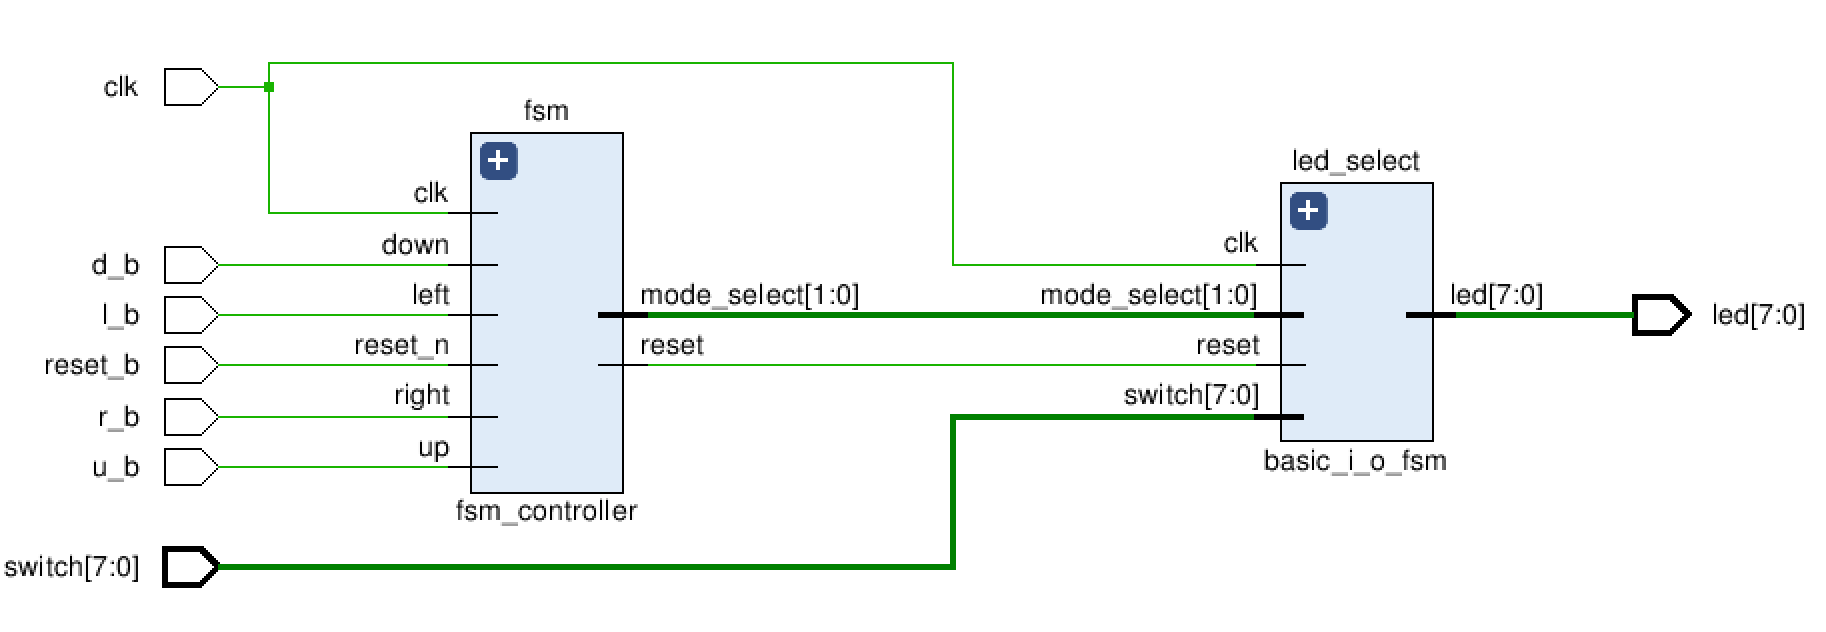
\includegraphics[scale=0.25]{img/partB.png}}
   \caption{Block Diagram for Part B}
   \label{figurelabel}
\end{figure}

\subsection{Entities}
\begin{table}[H]
\begin{tabular}{|l|l|}
\hline
\rowcolor[HTML]{EFEFEF} 
Entity      & Description                           \\ \hline
top & This is the hardware top level that \\ &connects the finite state machine to basic\_i\_o. \\ \hline
fsm\_controller &  This is the finite state machine that keeps track \\ &of the current state,  holds next state logic,  and \\& sends control signals to the basic\_i\_o module. \\ \hline
basic\_i\_o & This module takes in the control logic \\& from the state machine and selects the correct \\& altered  switch data to send to the LEDs. \\ \hline
\end{tabular}
\end{table}

\subsection{Design}
When designing this part of the MP, we first considered a design where the mode would only be selected when the push button was held down. We realized this was not the best approach. We then switched to a design were a mode was locked in when we pressed the push button. This lead to a more extensive state machine but the state control logic was still the same. 

\subsection{Performance}
This was a very small design and it took up very little resources on the Zinq 7000. The usage is shown in the table below. Figure 4 shows how the design was implemented on the device.
\begin{table}[H]
\centering
\caption{Resource Usage Part B}
\label{table_example}
\begin{tabular}{|l|r|r|r|}
\hline
\rowcolor[HTML]{EFEFEF} 
Resource & \multicolumn{1}{l|}{\cellcolor[HTML]{EFEFEF}Utilization} & \multicolumn{1}{l|}{\cellcolor[HTML]{EFEFEF}Available} & \multicolumn{1}{l|}{\cellcolor[HTML]{EFEFEF}Utilization \%} \\ \hline
LUT      & 22                                                        & 53200                                                  & 0.04                                                        \\ \hline
FF       & 11                                                       & 106400                                                 & 0.01                                                        \\ \hline
IO       & 22                                                       & 200                                                    & 11.00                                                        \\ \hline
BUFG     & 1                                                        & 32                                                     & 3.13                                                        \\ \hline
\end{tabular}
\end{table}

\begin{figure}[thpb]
   \centering
   \parbox{3in}{\centering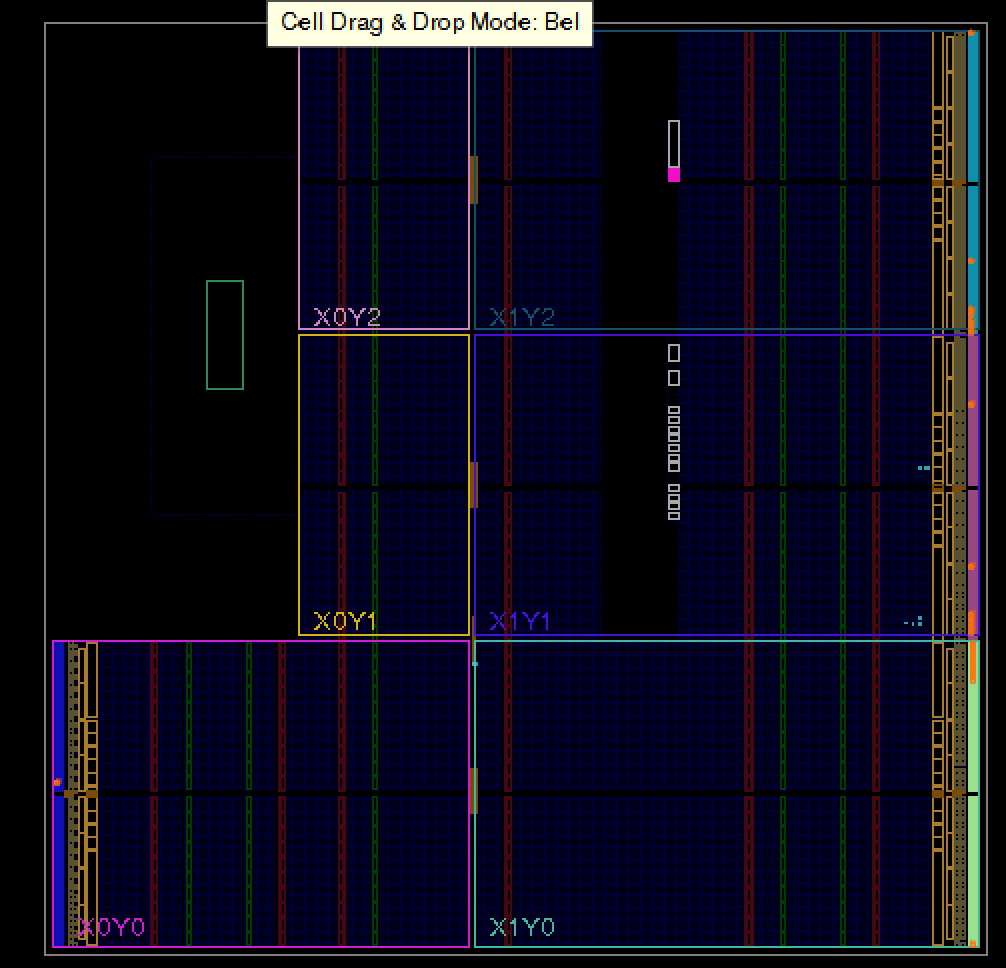
\includegraphics[scale=0.35]{img/partb_chip.png}}
   \caption{Device Mapping for Part B}
   \label{figurelabel}
\end{figure}

Because this design was also small,  most of the power consumed by the device was static power. 
\begin{table}[]
\centering
\caption{Resource Usage Part B}
\label{table_example}
\begin{tabular}{|l|r|}
\hline
\rowcolor[HTML]{EFEFEF} 
Type    & \multicolumn{1}{l|}{\cellcolor[HTML]{EFEFEF}Power} \\ \hline
Static  & 0.122 W                                            \\ \hline
Dynamic & 0.009 W                                            \\ \hline
\textbf{Total} & \textbf{0.131 W}                            \\ \hline
\end{tabular}
\end{table}


\begin{table}[]
\centering
\caption{Timing Report Part B}
\label{table_example}
\begin{tabular}{|l|l|}
\hline
\rowcolor[HTML]{EFEFEF} 
Type    & Time \\ \hline
Worst Hold Slack  &  0.253ns  \\ \hline
Worst Negative Slack & 0.7.47ns \\ \hline
Worst Pulse Width Slack & 4.5 ns \\ \hline
\end{tabular}
\end{table}






\subsection{Difficulites/Bugs}
For this part of the MP, the biggest difficulty was using the Verilog syntax of a finite state machine. After finding some resources online, the rest of this part was straightforward. 






\section{Part C}
\subsection{Description}
For the third part of the MP we had to interface the embedded ARM core with the switches and LEDs through the AXI bus and imitating the behavior of part B in software. The objective of this part was to familiarize ourselves with the process creating custom IP modules and writing software to interface with them.

\subsection{Assumptions}
The one assumption we made for this part of the MP is that during the modes a change in the switches will be reflected in the LEDs.

\subsection{System Configuration}
The Zynq 7000's integrated ARM cores interface with the switches and LEDs through a GPIO AXI port. The AXI interface block has two 8 bit channels and are directly connected to the switches and the LEDs. The block diagram of the configuration is shown in figure 3. When the GPIO module is created the Xilinx toolkit will automatically connect the modules for you and instantiate some supporting hardware. The toolkit automatically instantiated a system reset block so that the cores can be reset, as well as an AXI interconnect to allow for multiple AXI modules to be connected.

\begin{figure}[thpb]
   \centering
   \parbox{3in}{\centering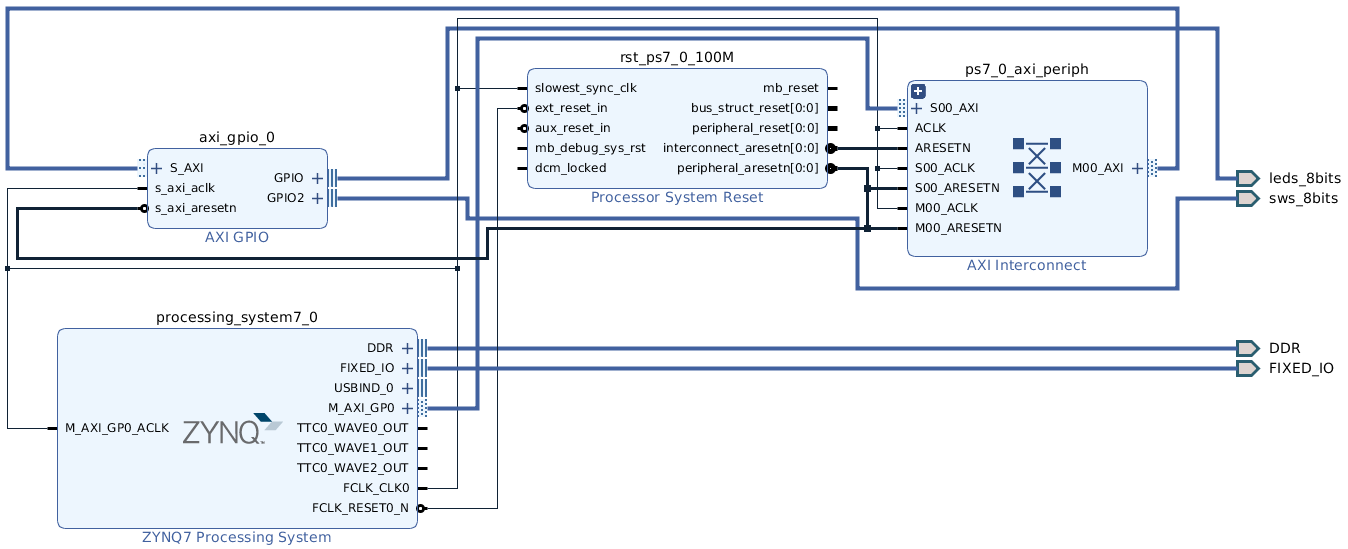
\includegraphics[scale=0.4]{img/mp1c_diagram.PNG}}
   \caption{Block Diagram for Part C}
   \label{figurelabel}
\end{figure}

A board support package, or BSP, is then generated from our hardware configuration. This allows the software development kit to understand what hardware it has access to and what memory locations the modules are located at. The software then interfaces through memory mapped I/O.

\subsection{Entities}
\begin{table}[H]
\centering
\begin{tabular}{|l|l|}
\hline
\rowcolor[HTML]{EFEFEF} 
Entity           & Description \\ \hline
Zinq7            & Main ARM core with\\ 
                 & interconnect and cache \\ \hline
AXI GPIO         & GPIO AXI module to\\
                 & interface with switches \\ \hline
System Reset     & Resets processor and \\ 
                 & connected devices \\ \hline
AXI Interconnect & Interconnect fabric for \\ 
                 & multiple AXI modules \\ \hline
\end{tabular}
\end{table}

\subsection{Design}
The other than instantiating a GPIO AXI module, the entire MP was done in software. The program looped through four distinct states spending about 1 second in each state. Within a state, the program sampled the state of the switches through DiscreteRead of the switch channel (channel 0) and then applied the operation for that state to the switch data. The data was then displayed on the LEDs though a DiscreteWrite to the LED channel (channel 1). The modes performed the same functions as Part B and the software flow chart is shown in figure 6.

\begin{figure}[thpb]
   \centering
   \parbox{3in}{\centering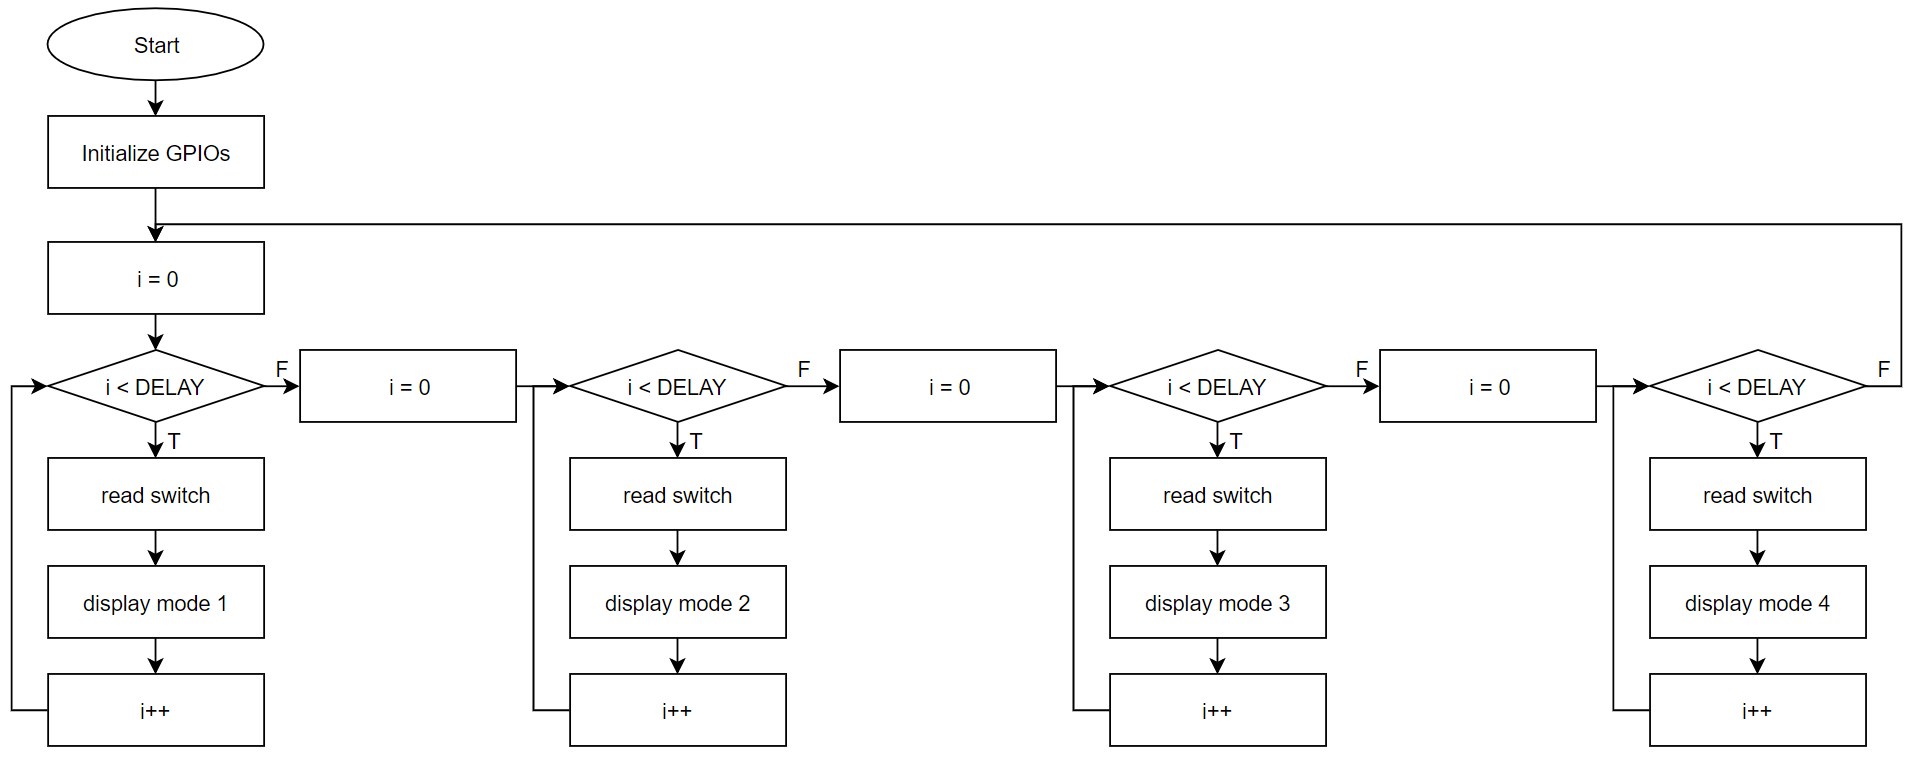
\includegraphics[scale=0.2]{img/program_flow_chart.PNG}}
   \caption{Program Flow for Part C}
   \label{figurelabel}
\end{figure}

We settled on the delay iterations number just by trial and error.

\subsection{Performance}
This a comparably larger design than the other two parts. The AXI GPIO module resided on the Programmable Logic fabric and that contained a lot of logic and registers. The AXI interface is a complex module so it occupied a lot of space after place and route (Figure 7).

\begin{table}[H]
\centering
\caption{Resource Usage Part C}
\label{table_example}
\begin{tabular}{|l|r|r|r|}
\hline
\rowcolor[HTML]{EFEFEF} 
Resource & \multicolumn{1}{l|}{\cellcolor[HTML]{EFEFEF}Utilization} & \multicolumn{1}{l|}{\cellcolor[HTML]{EFEFEF}Available} & \multicolumn{1}{l|}{\cellcolor[HTML]{EFEFEF}Utilization \%} \\ \hline
LUT      & 423                                                        & 53200                                                  & 0.80                                                        \\ \hline
LUTRAM   & 63                                                        & 17400 & 0.36                                                        \\ \hline

FF       & 648                                                       & 106400                                                 & 0.61                                                        \\ \hline
IO       & 16                                                       & 200                                                    & 8.00                                                        \\ \hline
BUFG     & 1                                                        & 32                                                     & 3.13                                                        \\ \hline
\end{tabular}
\end{table}

\begin{figure}[thpb]
   \centering
   \parbox{3in}{\centering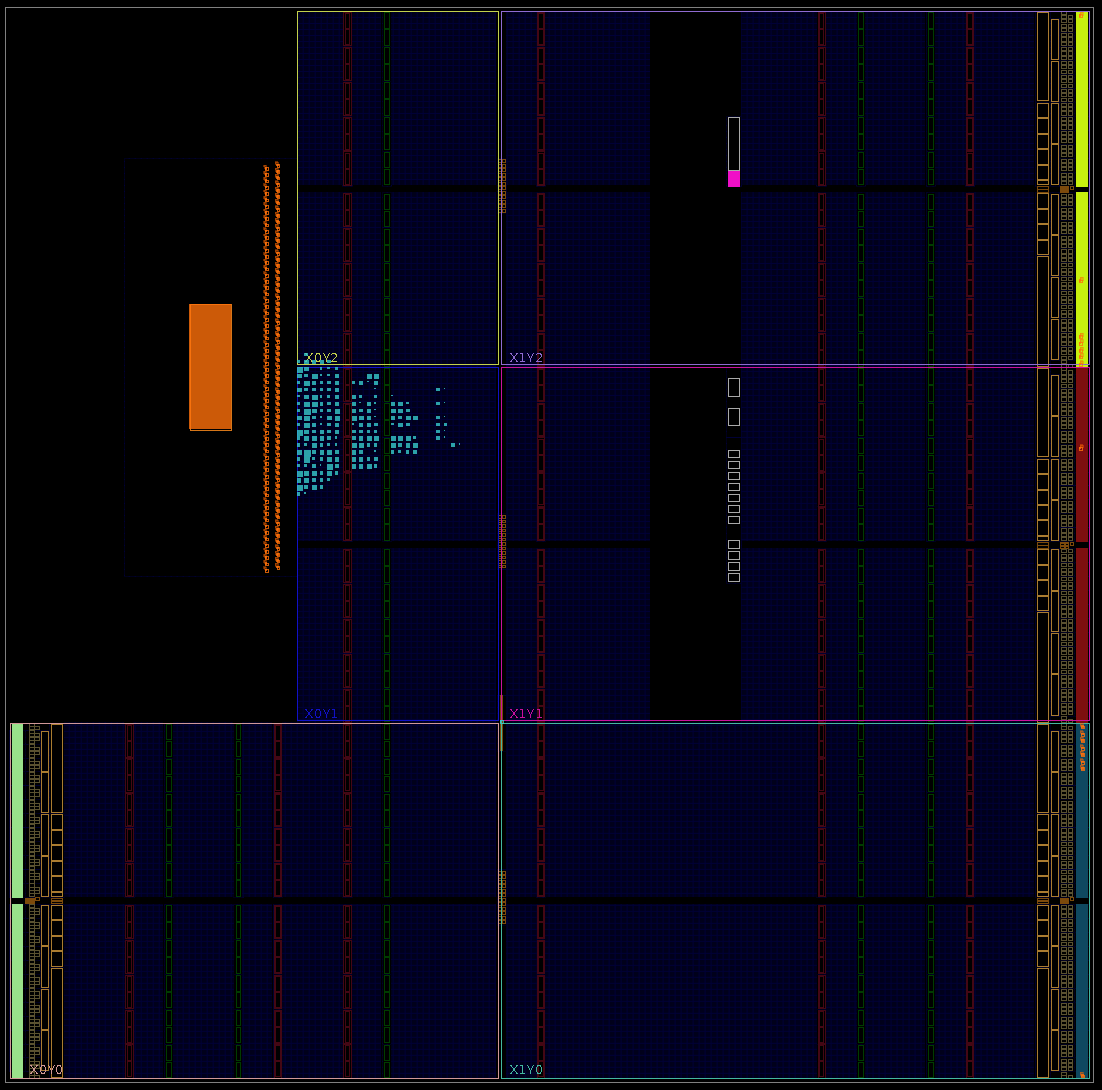
\includegraphics[scale=0.35]{img/mp1c_device.PNG}}
   \caption{Device Mapping for Part C}
   \label{figurelabel}
\end{figure}

This design incorporates the PS7 core which will constantly be consuming dynamic power as it loops through the program which is why the dynamic power is dramatically larger than the static power consumed. This desing is also larger than the others using more on chip resources which is also a reason the power has dramatically increased.

\begin{table}[H]
\centering
\caption{Resource Usage Part C}
\label{table_example}
\begin{tabular}{|l|r|}
\hline
\rowcolor[HTML]{EFEFEF} 
Type    & \multicolumn{1}{l|}{\cellcolor[HTML]{EFEFEF}Power} \\ \hline
Static  & 0.154 W                                            \\ \hline
Dynamic & 1.535 W                                            \\ \hline
\textbf{Total} & \textbf{1.689 W}                            \\ \hline
\end{tabular}
\end{table}

Again the design was very small so the place and route tool had no problem meeting the timing constraints. There are very reasonable worst setup and hold times for our design.

\begin{table}[H]
\centering
\caption{Timing Report Part C}
\label{table_example}
\begin{tabular}{|l|l|}
\hline
\rowcolor[HTML]{EFEFEF} 
Type                 & Time     \\ \hline
Worst Hold Slack     & 0.045 ns \\ \hline
Worst Negative Slack & 4.292 ns \\ \hline
Worst Pulse Width Slack & 4.020 ns \\ \hline
\end{tabular}
\end{table}

\subsection{Difficulties/Bugs}
The only difficulty encountered in this section was generating board support packages and making sure the package was up to date with the hardware. We had ran into issues where the BSP did not match the hardware that was loaded on the FPGA. 

\section{What We Learned}
At the start of this machine problem, we were introduced to the Xilinix program Vivado. After developing a simple design which dealt with basic input and output devices on the board, we moved onto a slightly larger design that used a finite state machine. Finally, we implemented a simple SoC using the Zynq system. This system taught us about block design automatons, AXI interfaces, and how to work with embedded software. 

\section{Environment}
We used Lubuntu 17.04 and 18.04 in a virtualbox virtual machine to do all of the work for this MP.


\end{document}
